\documentclass[11pt,a4paper,dvipsnames]{article}

\usepackage[top=2.5cm, bottom=2.5cm, left=2.8cm, right=2.8cm]{geometry}
\usepackage{amsmath}
\usepackage{booktabs}
\usepackage{array}
\usepackage{xcolor}
\usepackage{tikz}
\usetikzlibrary{arrows.meta, positioning, shapes.geometric, calc, backgrounds, fit}
\usepackage{hyperref}
\usepackage{microtype}
\usepackage{enumitem}
\usepackage{titlesec}
\usepackage{parskip}
\usepackage{tocloft}
\usepackage{fancyhdr}
\usepackage{lmodern}
\usepackage[T1]{fontenc}

% ── Colours ──────────────────────────────────────────────────────────────────
\definecolor{protoblue}{HTML}{1a4f7a}
\definecolor{protolight}{HTML}{daeaf6}
\definecolor{tealclaim}{HTML}{148a6e}
\definecolor{grayfill}{HTML}{f0f4f8}
\definecolor{tablehead}{HTML}{1a4f7a}
\definecolor{rulecolor}{HTML}{1a4f7a}


% ── Section formatting ────────────────────────────────────────────────────────
\titleformat{\section}
  {\large\bfseries\color{protoblue}}
  {\thesection}{1em}{}[\color{rulecolor}\titlerule]
\titleformat{\subsection}
  {\normalsize\bfseries\color{protoblue}}
  {\thesubsection}{1em}{}
\titlespacing{\section}{0pt}{1.4em}{0.6em}
\titlespacing{\subsection}{0pt}{1em}{0.4em}

% ── Lists ─────────────────────────────────────────────────────────────────────
\setlist[itemize]{itemsep=2pt,topsep=4pt,leftmargin=1.4em}
\setlist[enumerate]{itemsep=2pt,topsep=4pt,leftmargin=1.6em}

% ── Header / footer ──────────────────────────────────────────────────────────
\pagestyle{fancy}
\fancyhf{}
\fancyhead[L]{\small\color{gray}N-Party Cyclic Atomic Swap Protocol}
\fancyhead[R]{\small\color{gray}\thepage}
\renewcommand{\headrulewidth}{0.3pt}

% ── Hyperlinks ────────────────────────────────────────────────────────────────
\hypersetup{
  colorlinks=true,
  linkcolor=protoblue,
  urlcolor=protoblue,
  pdfauthor={},
  pdftitle={N-Party Cyclic Atomic Swap Protocol Specification}
}

% ── ToC formatting ────────────────────────────────────────────────────────────
\renewcommand{\cftsecfont}{\bfseries\color{protoblue}}
\renewcommand{\cftsecpagefont}{\bfseries\color{protoblue}}

% ── Convenience ──────────────────────────────────────────────────────────────
\newcommand{\msg}[1]{\textsf{#1}}
\newcommand{\var}[1]{\mathit{#1}}
\newcommand{\tagg}{t_{\mathrm{agg}}}
\newcommand{\Tagg}{T_{\mathrm{agg}}}
\newcommand{\Xagg}{X_{\mathrm{agg}}}
\newcommand{\Ragg}{R_{\mathrm{agg}}}

% ─────────────────────────────────────────────────────────────────────────────
\begin{document}

% ── Title page ───────────────────────────────────────────────────────────────
\begin{titlepage}
\centering
\vspace*{2.5cm}
{\huge\bfseries\color{protoblue}
  N-Party Cyclic Atomic Swap\\[0.4em]
  Protocol Specification\par}
\vspace{1.2cm}
\color{rulecolor}\rule{0.8\textwidth}{1.2pt}

\vspace{0.8cm}
{\large\color{black}
  A protocol description\par}
\vspace{0.5cm}
\color{rulecolor}\rule{0.8\textwidth}{0.4pt}
\vfill
{\normalsize\color{gray}\today}
\end{titlepage}

% ── Table of contents ─────────────────────────────────────────────────────────
\tableofcontents
\newpage

% ─────────────────────────────────────────────────────────────────────────────
\section{Setting}

A finite set of $N$ parties $P = \{P_0, P_1, \ldots, P_{N-1}\}$.
The party $P_0$ is the designated \textbf{leader}.

\subsection{Cycle}

The parties are arranged in a directed cycle:
\[
  P_0 \to P_1 \to P_2 \to \cdots \to P_{N-1} \to P_0.
\]
Each directed edge defines one \textbf{transfer}.

\subsection{Transfers}

$\mathbf{Transfer}_i$ is the transfer from $P_i$ to $P_{(i+1)\bmod N}$,
for $i = 0, \ldots, N-1$.

\medskip\noindent\textbf{Roles.}\;
Because the swap is cyclic, \emph{every} party plays all three of the
following roles simultaneously:

\begin{itemize}
  \item \textbf{Depositor} for $\mathrm{transfer}_i$: $P_i$ locks funds
    on-chain and, in Setup, drives the transaction-signing round.
  \item \textbf{Claimant} for $\mathrm{transfer}_{i-1}$: $P_i$ drives the
    key-exchange rounds of Setup and later claims the locked funds.
  \item \textbf{Co-signer} for all $N$ transfers: $P_i$ contributes its
    public key, nonce, and partial pre-signature to the multi-sig lock of
    every transfer's locked account.
\end{itemize}

\noindent
The terms \emph{sender} and \emph{receiver} are used below only as shorthand
for the depositor and claimant roles \emph{within a specific transfer}.
They do not denote distinct categories of party.

The leader $P_0$ is the claimant in $\mathrm{transfer}_{N-1}$ (the transfer
from $P_{N-1}$ to $P_0$).
Until the Claim phase, all parties execute identical protocol steps, differing
only in which transfer index they are depositing into and claiming from.
\textbf{The only asymmetry in the protocol is in the Claim phase}
(Section~\ref{sec:claim}), where the leader's behaviour diverges from that of
all other parties.

\bigskip
Figure~\ref{fig:cycle} shows the structure for $N = 3$.

\begin{figure}[h]
\centering
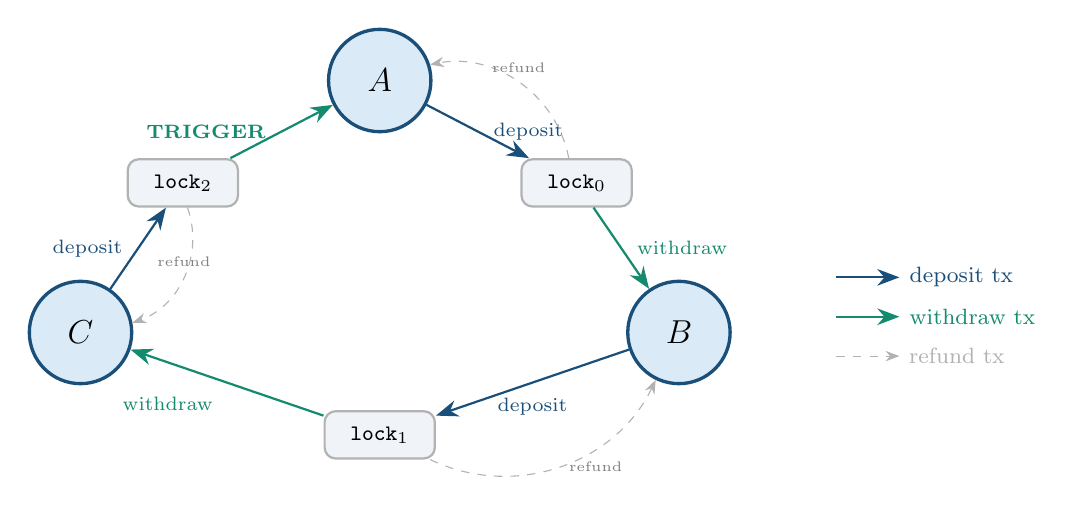
\begin{tikzpicture}[
  party/.style={
    circle, draw=protoblue, fill=protolight,
    very thick, minimum size=1.3cm, font=\bfseries\large},
  locked/.style={
    rectangle, rounded corners=4pt,
    draw=gray!60, fill=grayfill,
    thick, minimum width=1.4cm, minimum height=0.6cm, font=\footnotesize},
  dep/.style={-{Stealth[length=8pt]}, thick, protoblue},
  wit/.style={-{Stealth[length=8pt]}, thick, tealclaim},
  ref/.style={-{Stealth[length=5pt]}, dashed, gray!60},
]
  \node[party] (A) at (0, 3.2) {$A$};
  \node[party] (B) at (3.8, 0) {$B$};
  \node[party] (C) at (-3.8, 0) {$C$};

  \node[locked] (L0) at (2.5, 1.9) {$\mathtt{lock}_0$};
  \node[locked] (L1) at (0, -1.3) {$\mathtt{lock}_1$};
  \node[locked] (L2) at (-2.5, 1.9) {$\mathtt{lock}_2$};

  % Deposit
  \draw[dep] (A) -- node[right=2pt, font=\scriptsize] {deposit} (L0);
  \draw[dep] (B) -- node[below=2pt, font=\scriptsize] {deposit} (L1);
  \draw[dep] (C) -- node[left=2pt, font=\scriptsize] {deposit} (L2);

  % Withdraw
  \draw[wit] (L0) -- node[right=2pt, font=\scriptsize, tealclaim] {withdraw} (B);
  \draw[wit] (L1) -- node[below left=2pt, font=\scriptsize, tealclaim] {withdraw} (C);
  \draw[wit] (L2) -- node[left=2pt, font=\scriptsize, tealclaim] {\textbf{TRIGGER}} (A);

  % Refund (dashed)
  \draw[ref] (L0) to[bend right=45]
    node[above, font=\tiny, gray] {refund} (A);
  \draw[ref] (L1) to[bend right=45]
    node[right, font=\tiny, gray] {refund} (B);
  \draw[ref] (L2) to[bend left=45]
    node[above, font=\tiny, gray] {refund} (C);

  % Legend
  \begin{scope}[shift={(5.8,-0.5)}]
    \draw[dep] (0,1.2) -- (0.8,1.2) node[right, font=\footnotesize] {deposit tx};
    \draw[wit] (0,0.7) -- (0.8,0.7) node[right, font=\footnotesize] {withdraw tx};
    \draw[ref] (0,0.2) -- (0.8,0.2) node[right, font=\footnotesize] {refund tx};
  \end{scope}
\end{tikzpicture}
\caption{Three-party cyclic swap ($N=3$, leader $= A$).
  Blue solid arrows: deposit path.
  Teal solid arrows: withdraw (claim) path.
  The \textbf{TRIGGER} is the first withdraw broadcast, by the leader $A$
  claiming $C$'s locked funds.
  Dashed arrows: refund path (time-locked, unhappy path only).}
\label{fig:cycle}
\end{figure}

% ─────────────────────────────────────────────────────────────────────────────
\section{Core Data}

\subsection{Aggregate Adaptor Secret}

Each party $P_i$ holds a private \textbf{adaptor secret} $t_i$.
The corresponding public \textbf{adaptor point} is $T_i = t_i \cdot G$,
where $G$ is the curve generator.
$T_i$ is broadcast to all parties at the start of the Setup phase.
The \textbf{aggregate adaptor point} $\Tagg$ is the sum of all individual
adaptor points. The corresponding \textbf{aggregate adaptor secret} is:
\[
  \tagg = t_0 + t_1 + \cdots + t_{N-1}.
\]
This single secret is used to complete the withdraw transaction for
\emph{every} transfer.
It is distributed: no strict subset of parties can compute it unilaterally.

\subsection{Transactions Per Transfer}

For each $\mathrm{transfer}_i$ three transactions are constructed during Setup:

\begin{center}
\renewcommand{\arraystretch}{1.3}
\begin{tabular}{@{}p{2.6cm}p{3cm}p{3.2cm}p{4.8cm}@{}}
\toprule
\textbf{Transaction} & \textbf{Spends} & \textbf{Produces} & \textbf{Authorisation} \\
\midrule
Deposit tx
  & $P_i$'s own funds
  & Locked account for $\mathrm{transfer}_i$
  & $P_i$'s signature alone \\[4pt]
Withdraw tx
  & Locked account
  & $P_{(i+1)\bmod N}$'s address
  & Aggregate multi-sig $+\ \tagg$ \\[4pt]
Refund tx
  & Locked account
  & $P_i$'s address
  & Aggregate multi-sig $+$ block $\geq W_i$ \\
\bottomrule
\end{tabular}
\end{center}

\noindent
The \textbf{withdraw tx} is constructed as a \emph{pre-signature} during Setup
and completed only during the Claim phase when $\tagg$ becomes known.
The \textbf{refund tx} is fully co-signed during Setup but is time-locked
and cannot be broadcast before block height $W_i$.

\subsection{Locked Account}

Each transfer's locked account is an $N$-of-$N$ multi-signature account.
Its unlocking key is an aggregated public key derived from all $N$ parties'
individual public keys. Spending it requires a single aggregated Schnorr
signature committing all $N$ parties.

\medskip\noindent\textbf{Mutual exclusion assumption.}\;
For each transfer's locked account, the underlying chain guarantees that at
most one of the withdraw tx and the refund tx can be confirmed.
In UTXO-based chains this holds structurally (spending a UTXO consumes it,
invalidating any other transaction that references it); other chain models
must enforce it explicitly.

\subsection{Refund Windows}
\label{sec:windows}

Each $\mathrm{transfer}_i$ has an associated \textbf{refund window open height}
$W_i$: the minimum block height of a chosen blockchain at which the refund tx for
$\mathrm{transfer}_i$ becomes valid.

\medskip
\noindent\textbf{Staggered window invariant (cyclic case):}
\[
  W_0\ >\ W_1\ >\ W_2\ >\ \cdots\ >\ W_{N-1}.
\]
The leader $P_0$'s refund window (for $\mathrm{transfer}_0$, the deposit made
by $P_0$) opens \textbf{last}.
$P_{N-1}$'s refund window (for the deposit into the leader) opens \textbf{first}.

\medskip
\noindent\textbf{Minimum gap requirement.}\;
Let $\Delta$ be the \textbf{claim propagation time}: the maximum number of
blocks required for a party to (1)~observe a broadcast transaction at the
required finality depth, (2)~construct and sign the corresponding withdraw
tx, and (3)~have it confirmed to the required finality depth.
The staggered ordering alone is not sufficient for safety; the gaps must
satisfy:
\[
  W_i - W_{i+1} \;\geq\; \Delta \qquad \text{for all } i = 0, \ldots, N-2.
\]
$\Delta$ is a protocol parameter that must be fixed before the Config phase
and depends on the confirmation-depth policies of the relevant blockchains.
This value \textbf{must be chosen conservatively} as the security of the protocol depends 
entirely on it.

\medskip
\noindent\textbf{Security note.}\;
If $W_i - W_{i+1} < \Delta$, a malicious leader (the only party that
controls the trigger broadcast) can allow $W_{i+1}$ to expire before
$P_{(i+1)\bmod N}$ can confirm its withdraw tx.
$P_{(i+1)\bmod N}$ then claims a refund, but the adversary also claims
$P_{(i+1)\bmod N}$'s deposit via the withdraw tx: that party loses their
deposit and receives nothing, breaking atomicity.

\medskip
\noindent\textbf{Griefing opportunity cost asymmetry.}\;
Because refund windows are staggered, an abort imposes unequal waiting
costs on different parties.
If any party aborts after the Lock phase, every party eventually recovers
their principal via the refund path; no principal is lost.
However, a party with a small $W_j$ (refund available early) that withholds
their adaptor secret forces the leader, who holds the largest window $W_0$,
to keep funds locked for the longest period.
The aborting party bears a shorter opportunity cost than the leader does.
This asymmetry is a liveness concern, not an atomicity violation.

\medskip
\noindent\textbf{Optionality.}\;
The temporal gap between the Lock phase (when all funds are committed) and
the leader's decision to broadcast the trigger creates a free option for
the leader.
During this gap the leader can observe price movements and choose to
complete the swap (if prices moved favourably) or let it expire via refund
(if prices moved against them).
The non-leader parties are locked in and cannot exit.
Han et al.~\cite{han2019optionality} prove that this is structurally
equivalent to a premium-free American call option granted to the leader at
the non-leaders' expense, and estimate the fair option premium at 2--3\%
of the swap value for typical cryptocurrency volatility.
The protocol does not require the leader to broadcast the trigger within
any deadline, nor does it impose a premium to compensate non-leaders for
this optionality.
The refund path ensures no principal is lost, but expected value is
transferred from non-leaders to the leader through the option itself.
This is not specific to this protocol: it is a structural property of all
atomic swap protocols (HTLC or adaptor-signature-based) in which one party
commits last.

\begin{figure}[h]
\centering
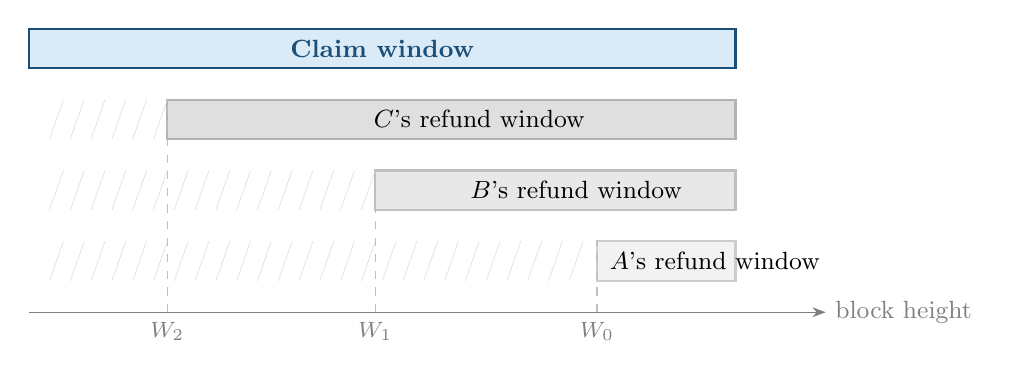
\begin{tikzpicture}[xscale=0.88, yscale=1.0]
  % Axis
  \draw[-{Stealth}, gray] (0,-0.3) -- (11.5,-0.3)
    node[right, font=\small] {block height};

  % Claim window (top bar)
  \fill[protolight] (0,2.8) rectangle (10.2,3.3);
  \draw[protoblue, thick] (0,2.8) rectangle (10.2,3.3);
  \node[font=\small\bfseries, protoblue] at (5.1,3.05) {Claim window};

  % C's refund (earliest, W2)
  \fill[gray!25] (2.0,1.9) rectangle (10.2,2.4);
  \draw[gray!60, thick] (2.0,1.9) rectangle (10.2,2.4);
  \draw[dashed, gray!50] (2.0,-0.3) -- (2.0,2.4);
  \node[below, font=\footnotesize, gray] at (2.0,-0.3) {$W_2$};
  \node[font=\small] at (6.5,2.15) {$C$'s refund window};

  % B's refund (W1)
  \fill[gray!18] (5.0,1.0) rectangle (10.2,1.5);
  \draw[gray!50, thick] (5.0,1.0) rectangle (10.2,1.5);
  \draw[dashed, gray!50] (5.0,-0.3) -- (5.0,1.5);
  \node[below, font=\footnotesize, gray] at (5.0,-0.3) {$W_1$};
  \node[font=\small] at (7.9,1.25) {$B$'s refund window};

  % A's refund (latest, W0)
  \fill[gray!10] (8.2,0.1) rectangle (10.2,0.6);
  \draw[gray!40, thick] (8.2,0.1) rectangle (10.2,0.6);
  \draw[dashed, gray!50] (8.2,-0.3) -- (8.2,0.6);
  \node[below, font=\footnotesize, gray] at (8.2,-0.3) {$W_0$};
  \node[font=\small] at (9.9,0.35) {$A$'s refund window};

  % Hatching before each window
  \foreach \x in {0.3,0.6,...,1.9} {
    \draw[gray!30, very thin] (\x,1.9) -- ++(0.2,0.5);
  }
  \foreach \x in {0.3,0.6,...,4.9} {
    \draw[gray!30, very thin] (\x,1.0) -- ++(0.2,0.5);
  }
  \foreach \x in {0.3,0.6,...,8.1} {
    \draw[gray!30, very thin] (\x,0.1) -- ++(0.2,0.5);
  }
\end{tikzpicture}
\caption{Staggered refund windows for $N=3$.
  $W_2 < W_1 < W_0$.
  The claim window is the period during which withdraw transactions may be
  broadcast.
  Hatched regions are the blocks before a party's refund window is active.}
\label{fig:windows}
\end{figure}

% ─────────────────────────────────────────────────────────────────────────────
\section{Protocol Phases}

Each transfer independently progresses through five phases.
Phases for different transfers run concurrently but are synchronised at two
global barriers (Lock and Claim, see Sections~\ref{sec:lock}
and~\ref{sec:claim}).

\begin{figure}[h]
\centering
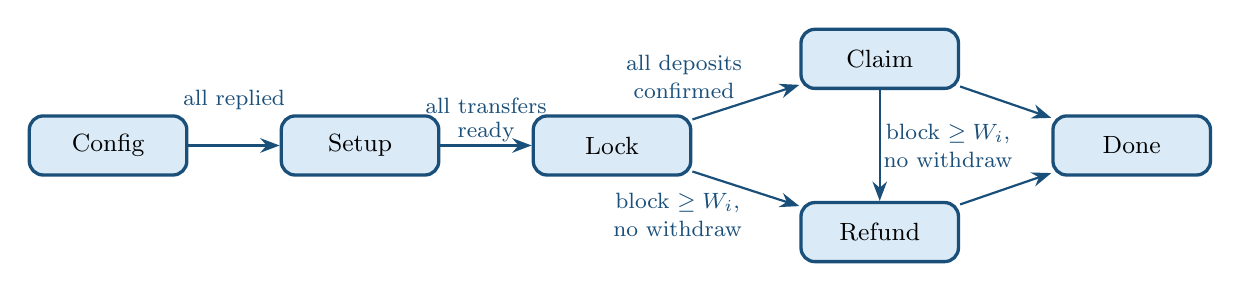
\begin{tikzpicture}[
  st/.style={
    rectangle, rounded corners=5pt,
    draw=protoblue, fill=protolight,
    very thick, minimum width=2.0cm, minimum height=0.75cm, font=\small},
  ar/.style={-{Stealth[length=7pt]}, thick, protoblue},
  lbl/.style={font=\footnotesize, inner sep=1pt},
]
  \node[st] (cfg)  at (0,0)    {Config};
  \node[st] (stp)  at (3.2,0)  {Setup};
  \node[st] (lck)  at (6.4,0)  {Lock};
  \node[st] (clm)  at (9.8,1.1){Claim};
  \node[st] (rfn)  at (9.8,-1.1){Refund};
  \node[st] (done) at (13.0,0) {Done};

  \draw[ar] (cfg) -- node[lbl,above] {\shortstack{all replied\\ \vspace{1em}}} (stp);
  \draw[ar] (stp) -- node[lbl,above] {\shortstack{all transfers\\ready}} (lck);
  \draw[ar] (lck) -- node[lbl,above left] {\shortstack{all deposits\\confirmed}} (clm);
  \draw[ar] (lck) -- node[lbl,below left] {\shortstack{block $\geq W_i$,\\no withdraw}} (rfn);
  \draw[ar] (clm) -- (done);
  \draw[ar] (clm) -- node[lbl,right] {\shortstack{block $\geq W_i$,\\no withdraw}} (rfn);
  \draw[ar] (rfn) -- (done);
\end{tikzpicture}
\caption{Phase state machine for a single transfer.
  The Lock$\,\to\,$Claim transition fires when the party has observed all
  $N$ deposits confirmed on-chain.
  The Lock$\,\to\,$Refund and Claim$\,\to\,$Refund transitions fire when
  the refund window opens and the withdraw tx has not yet been broadcast.}
\label{fig:phases}
\end{figure}

\noindent\textbf{Local synchronisation conditions:}
\begin{itemize}
  \item A party enters \textbf{Lock} only after it has completed all four
    Setup rounds for every transfer.
  \item A party enters \textbf{Claim} only after it has observed all $N$
    deposit txs confirmed on-chain at the required finality depth.
\end{itemize}

% ─────────────────────────────────────────────────────────────────────────────
\section{Config Phase}

\textbf{Goal.}\;
Establish the swap parameters, have each party generate its private adaptor
secret, and confirm that all $N$ parties are willing to proceed before any
cryptographic material is exchanged between parties.

\medskip\noindent
Config has two parts: a one-time global step and a per-transfer consent step.

\medskip\noindent\textbf{Part 1 — Swap description (once per swap).}\;
The swap initiator distributes the \textbf{swap description} to all $N$
parties: a unique swap identifier, the ordered party list
$[P_0, \ldots, P_{N-1}]$, the leader's identity, and the proposed refund
window heights $W_0, \ldots, W_{N-1}$.
Each party $P_i$ records $\var{swap\_id}$, $\var{parties}$, and
$\var{leader} = P_0$, and generates its private \textbf{adaptor secret}
$t_i$ uniformly at random.

\medskip\noindent\textbf{Part 2 — Per-transfer consent.}\;
For $\mathrm{transfer}_i$, $P_{(i+1)\bmod N}$ proposes the swap description
to all $N$ parties; each party either accepts or withholds consent.
$P_{(i+1)\bmod N}$ proceeds to Setup only after receiving consent from all
$N$ parties.

\noindent\textbf{Pre-condition (for a party to consent):}
\begin{itemize}
  \item The party has received the swap description: the transfer cycle, the
    complete ordered party list, the leader's identity, and the proposed
    refund window heights $W_0, \ldots, W_{N-1}$.
  \item The proposed windows satisfy the staggered invariant
    $W_0 > W_1 > \cdots > W_{N-1}$ with gaps $W_i - W_{i+1} \geq \Delta$.
\end{itemize}

\noindent\textbf{Post-condition:}
Every party holds the swap description and its own private adaptor secret
$t_i$.
All $N$ parties have agreed on the swap description and $P_{(i+1)\bmod N}$
may proceed to Setup for $\mathrm{transfer}_i$.

% ─────────────────────────────────────────────────────────────────────────────
\section{Setup Phase}

\textbf{Goal.}\;
Construct and mutually verify all three transactions for every transfer so
that:
\begin{enumerate}
  \item Everyone can independently compute $\Tagg$.
  \item For each $\mathrm{transfer}_i$, $P_{(i+1)\bmod N}$ holds a verified
    pre-signature for the withdraw tx (completable once $\tagg$ is known, and
    not before).
  \item For each $\mathrm{transfer}_i$, $P_i$ holds a fully co-signed,
    time-locked refund tx.
  \item All parties have verified that every refund window $W_i$ is correctly
    set.
\end{enumerate}

\medskip\noindent
Setup begins with a one-time preliminary step in which every party broadcasts
its individual adaptor point $T_i$ to all other parties.
This happens once per swap, before any per-transfer rounds begin.

The per-transfer rounds then run once for each transfer and every party
participates in every instance.
For $\mathrm{transfer}_i$, the four rounds are structured as follows:
Rounds~1--3 are initiated by $P_{(i+1)\bmod N}$ in its claimant role;
Round~4 is initiated by $P_i$ in its depositor role.
All $N$ parties respond in every round for every transfer.
Since there are $N$ transfers, each party initiates Rounds~1--3 exactly once,
initiates Round~4 exactly once, and responds in all four rounds $N$ times.
Figure~\ref{fig:setup} shows the per-transfer sub-protocol.

\begin{figure}[h]
\centering
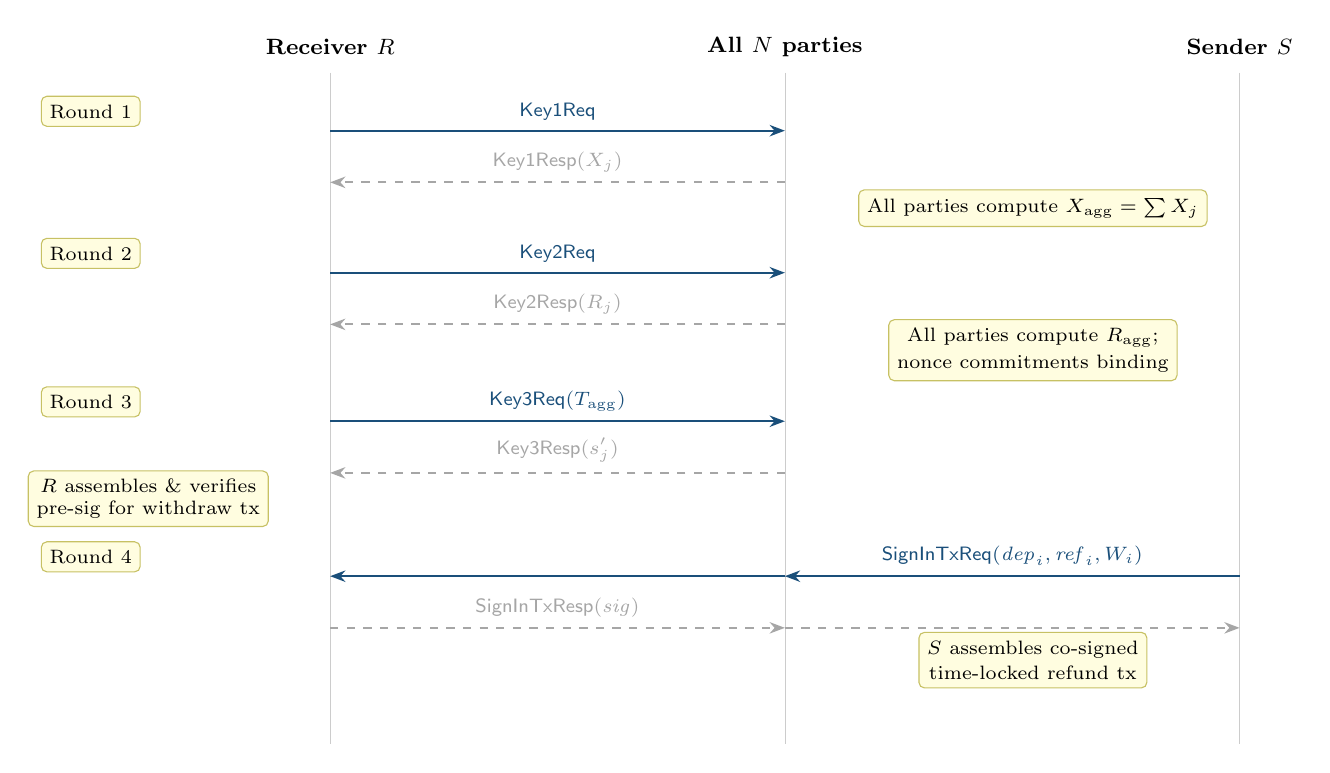
\begin{tikzpicture}[
  xscale=1.05, yscale=0.82,
  life/.style={very thin, gray!40},
  fwd/.style={-{Stealth[length=5.5pt]}, thick, protoblue},
  bwd/.style={-{Stealth[length=5.5pt]}, thick, dashed, gray!70},
  note/.style={
    font=\scriptsize, fill=yellow!12, draw=yellow!50!gray,
    rounded corners=2pt, inner sep=3pt},
  hdr/.style={font=\footnotesize\bfseries},
]
  % Column headers and lifelines
  \node[hdr] (R)   at (0,0)   {Receiver $R$};
  \node[hdr] (ALL) at (5.5,0) {All $N$ parties};
  \node[hdr] (S)   at (11,0)  {Sender $S$};
  \draw[life] (0,-0.4)   -- (0,-10.8);
  \draw[life] (5.5,-0.4) -- (5.5,-10.8);
  \draw[life] (11,-0.4)  -- (11,-10.8);

  % ── Round 1 ──────────────────────────────────────────────────────────
  \node[note, anchor=west] at (-3.5,-1) {Round 1};
  \draw[fwd] (0,-1.3)  -- node[above,font=\scriptsize] {\msg{Key1Req}} (5.5,-1.3);
  \draw[bwd] (5.5,-2.1) -- node[above,font=\scriptsize] {\msg{Key1Resp}$(X_j)$} (0,-2.1);
  \node[note] at (8.5,-2.5) {All parties compute $\Xagg = \sum X_j$};

  % ── Round 2 ──────────────────────────────────────────────────────────
  \node[note, anchor=west] at (-3.5,-3.2) {Round 2};
  \draw[fwd] (0,-3.5)  -- node[above,font=\scriptsize] {\msg{Key2Req}} (5.5,-3.5);
  \draw[bwd] (5.5,-4.3) -- node[above,font=\scriptsize] {\msg{Key2Resp}$(R_j)$} (0,-4.3);
  \node[note] at (8.5,-4.7) {\shortstack{All parties compute $\Ragg$;\\nonce commitments binding}};

  % ── Round 3 ──────────────────────────────────────────────────────────
  \node[note, anchor=west] at (-3.5,-5.5) {Round 3};
  \draw[fwd] (0,-5.8)  -- node[above,font=\scriptsize] {\msg{Key3Req}$(\Tagg)$} (5.5,-5.8);
  \draw[bwd] (5.5,-6.6) -- node[above,font=\scriptsize] {\msg{Key3Resp}$(s'_j)$} (0,-6.6);
  \node[note] at (-2.2,-7.0) {\shortstack{$R$ assembles \& verifies\\pre-sig for withdraw tx}};

  % ── Round 4 ──────────────────────────────────────────────────────────
  \node[note, anchor=west] at (-3.5,-7.9) {Round 4};
  \draw[fwd] (11,-8.2) -- node[above,font=\scriptsize] {\msg{SignInTxReq}$(\mathit{dep}_i, \mathit{ref}_i, W_i)$} (5.5,-8.2);
  \draw[fwd] (5.5,-8.2) -- (0,-8.2);
  \draw[bwd] (0,-9.0)  -- node[above,font=\scriptsize] {\msg{SignInTxResp}$(\mathit{sig})$} (5.5,-9.0);
  \draw[bwd] (5.5,-9.0) -- (11,-9.0);
  \node[note] at (8.5,-9.5) {\shortstack{$S$ assembles co-signed\\time-locked refund tx}};
\end{tikzpicture}
\caption{Setup per-transfer sub-protocol sequence.
  The preliminary adaptor point broadcast (once per swap, before these rounds)
  is described in \S\ref{sec:setup-prelim}.
  Rounds 1--3: receiver-driven key and pre-signature exchange.
  Round~4: sender-driven transaction signing.
  Each \msg{Key$k$Req} is broadcast to all $N$ parties; responses return to
  the initiator.}
\label{fig:setup}
\end{figure}

\subsection{Preliminary — Adaptor Point Broadcast}
\label{sec:setup-prelim}

This step runs \textbf{once per swap}, before any per-transfer rounds begin.

Every party $P_j$ computes its \textbf{adaptor point} $T_j = t_j \cdot G$
from its private adaptor secret $t_j$, and broadcasts $T_j$ to all $N$ parties.
All parties store the full set $\{T_0, T_1, \ldots, T_{N-1}\}$ for later use
in Round~3.

\noindent\textbf{Pre-condition:} Config complete for all transfers.\\
\noindent\textbf{Post-condition:} Every party holds the individual adaptor
points $T_j$ for all $j$ and can independently compute the aggregate adaptor
point $\Tagg = T_0 + T_1 + \cdots + T_{N-1}$.
If any party withholds or sends a malformed $T_j$, the discrepancy is
detected no later than Round~3, when co-signers independently verify
$\Tagg$ against the individual adaptor points.

% ─────────────────────────────────────────────────────────────────────────────

\subsection{Round 1 — Public Key Exchange (\msg{Key1})}

\textbf{Initiator for $\mathrm{transfer}_i$:}
$P_{(i+1)\bmod N}$ broadcasts \msg{Key1Req} to all $N$ parties.

Every party $P_j$ responds with its \textbf{public key} $X_j$.
All parties compute the \textbf{aggregated public key}
$\Xagg = X_0 + X_1 + \cdots + X_{N-1}$,
which determines the locked account address for $\mathrm{transfer}_i$.

\noindent\textbf{Pre-condition:} Preliminary step complete; Config complete for $\mathrm{transfer}_i$.\\
\textbf{Post-condition:} All parties agree on $\Xagg$ and hence on the locked
account address for $\mathrm{transfer}_i$.

\subsection{Round 2 — Nonce Exchange (\msg{Key2})}

\textbf{Initiator for $\mathrm{transfer}_i$:}
$P_{(i+1)\bmod N}$ broadcasts \msg{Key2Req} to all $N$ parties.

Every party $P_j$ responds with its \textbf{public nonce} $R_j$.
All parties compute the \textbf{aggregate nonce}
$\Ragg = R_0 + \cdots + R_{N-1}$.

\noindent\textbf{Pre-condition:} Round~1 complete for $\mathrm{transfer}_i$.\\
\textbf{Post-condition:} All parties are committed to a specific nonce for
partial signature computation for $\mathrm{transfer}_i$.
Changing a nonce after this point invalidates all collected partial
signatures, making the commitment binding by construction.

\subsection{Round 3 — Pre-signature Exchange (\msg{Key3})}

\textbf{Initiator for $\mathrm{transfer}_i$:}
$P_{(i+1)\bmod N}$ broadcasts \msg{Key3Req} together with the claimed
aggregate adaptor point $\Tagg$ to all $N$ parties.

Before computing its partial pre-signature, each responding party
\textbf{must verify}:
\begin{itemize}
  \item $\Tagg = T_0 + T_1 + \cdots + T_{N-1}$, computed independently
    from the individual adaptor points $T_j$ broadcast in the Preliminary
    step of Setup.
  \item The withdraw tx being pre-signed spends the correct locked account
    (the address determined by $\Xagg$ in Round~1) and credits
    $P_{(i+1)\bmod N}$'s address for the agreed amount.
\end{itemize}

\noindent\textbf{Security note.}\;
If co-signers do not verify $\Tagg$, the initiating party can substitute
$\Tagg' = \Tagg + \delta \cdot G$ for an arbitrary scalar $\delta$.
The resulting pre-signature requires $\tagg + \delta$ to complete.
That value is extractable on-chain after the trigger, but it is not
$\tagg$; all other parties' withdraw transactions, which require $\tagg$,
become permanently invalid, and the initiating party alone can claim.

Every responding party $P_j$ computes its \textbf{partial pre-signature}
$s'_j$ over the (verified) withdraw tx for $\mathrm{transfer}_i$ and sends
it to $P_{(i+1)\bmod N}$.
$P_{(i+1)\bmod N}$ assembles the \textbf{aggregate pre-signature} from all
$N$ responses and verifies it against the (verified) $\Tagg$.

\noindent\textbf{Pre-condition:} Round~2 complete; all parties hold the
individual adaptor points $T_j$ for all $j$ (broadcast in the Preliminary step).\\
\textbf{Post-condition:} $P_{(i+1)\bmod N}$ holds a verified aggregate
pre-signature for the withdraw tx of $\mathrm{transfer}_i$.
This pre-signature is not a valid signature; it becomes one if and only if
$\tagg$ is applied to it.
No party can complete this withdraw tx without knowing $\tagg$.

\subsection{Round 4 — Input Transaction Signing (\msg{SignInTx})}

\textbf{Initiator for $\mathrm{transfer}_i$:}
$P_i$ broadcasts \msg{SignInTxReq} containing the proposed
\textbf{deposit transaction} $\mathit{dep}_i$, the proposed
\textbf{refund transaction} $\mathit{ref}_i$, and the claimed refund window
height $W_i$.

Before co-signing, each party \textbf{must verify all of the following}:
\begin{itemize}
  \item The deposit tx sends funds to the locked account address determined
    by $\Xagg$ in Round~1 (not a substituted address).
  \item The deposit tx amount matches the agreed transfer amount for
    $\mathrm{transfer}_i$.
  \item The refund tx spends the correct locked account for
    $\mathrm{transfer}_i$.
  \item The refund tx credits $P_i$'s address.
  \item The refund tx time-lock is exactly $W_i$.
  \item $W_i$ is consistent with the window heights agreed in the Config
    phase and satisfies the staggered invariant
    ($W_{i-1} > W_i > W_{i+1}$, with boundary conditions at
    $i = 0$ and $i = N-1$).
\end{itemize}

\noindent\textbf{Security note.}\;
Without these checks, a malicious depositor can present a deposit tx that
sends to an attacker-controlled address, or a refund tx with a shortened
time-lock, and obtain co-signatures on it from all other parties.
A mis-addressed deposit tx allows the attacker to claim the locked funds
directly; a shortened refund lock allows a refund before the claim window
closes, in both cases forfeiting the rightful claimant's output.

A party that fails any of the above checks withholds its
\msg{SignInTxResp}, causing Setup to stall; that party waits for its refund
window to open and broadcasts its refund tx.

$P_i$ assembles the fully co-signed refund tx from all $N$ responses.

\noindent\textbf{Pre-condition:} Round~3 complete for $\mathrm{transfer}_i$.

\noindent\textbf{Post-condition ($P_i$):} Holds the deposit tx (ready to
broadcast) and a fully co-signed time-locked refund tx valid at block height
$\geq W_i$.

\noindent\textbf{Post-condition (all parties):} Have verified the deposit tx
destination, the refund tx recipient and time-lock, and the refund window
$W_i$ against the agreed protocol parameters.

% ─────────────────────────────────────────────────────────────────────────────
\section{Lock Phase}
\label{sec:lock}

\textbf{Goal.}\;
All senders deposit their funds into their respective locked accounts
on-chain.

\textbf{Pre-condition:}
The party has completed all four Setup rounds for all $N$ transfers and has
verified pre-signatures and refund windows for every transfer.
A party does not lock funds unless satisfied that it can either claim its
output or obtain a refund.

\noindent\textbf{Actions:}
\begin{enumerate}
  \item Every party $P_i$ broadcasts its deposit tx for $\mathrm{transfer}_i$.
  \item All parties monitor all blockchains and wait for finality of all $N$
    deposit txs.
\end{enumerate}

\noindent\textbf{Post-condition:}
For each $\mathrm{transfer}_i$, the locked account holds $P_i$'s funds.
The only ways to spend those funds are:
(a)~the withdraw tx (requiring $\tagg$), or
(b)~the refund tx (after block $W_i$, with the already co-signed multi-sig).

% ─────────────────────────────────────────────────────────────────────────────
\section{Claim Phase}
\label{sec:claim}

\textbf{Goal.}\;
Every party claims the funds locked for the transfer it is receiving.

\textbf{Pre-condition:}
The party has observed all $N$ deposit txs confirmed on-chain at the
required finality depth.

\medskip\noindent
\textbf{This is the only phase where parties are treated differently.}
Up to this point the protocol has been fully symmetric: every party has acted
as co-signer for all $N$ transfers, driven Rounds~1--3 for exactly one
transfer, and driven Round~4 for exactly one transfer.
The Claim phase breaks this symmetry solely through the role of the leader
$P_0$, whose behaviour diverges from that of all other parties as described
below.

\subsection{Leader's Role ($P_0$)}

\begin{enumerate}
  \item $P_0$ solicits adaptor secrets $t_j$ from each non-leader party $P_j$
    ($j = 1, \ldots, N{-}1$) over a private off-chain channel.
  \item Each non-leader party $P_j$ sends $t_j$ to $P_0$ \textbf{only after}
    independently confirming that all $N$ deposits are finalised on-chain.
  \item $P_0$ receives $t_j$ from each $P_j$ and verifies it against the
    corresponding public adaptor point $T_j$.
  \item $P_0$ computes $\tagg = t_0 + t_1 + \cdots + t_{N-1}$, completes the
    pre-signature for the withdraw tx of $\mathrm{transfer}_{N-1}$, and
    broadcasts it --- the \textbf{trigger transaction}.
\end{enumerate}

\noindent\textbf{Deviation --- withheld or malformed secret.}\;
If any $P_j$ withholds $t_j$, or the received value does not verify against
$T_j$, $P_0$ cannot assemble $\tagg$ and does not broadcast the trigger.
All parties fall through to the \textbf{Refund phase}: each party $P_i$ waits
until block height $\geq W_i$ and broadcasts their refund tx.
No party loses funds because refund txs were fully co-signed during Setup.

\medskip\noindent\textbf{Critical constraint.}\;
$P_0$ must \textbf{never} share $t_0$ off-chain.
$P_0$'s adaptor secret is disclosed only through the on-chain broadcast of
the trigger tx.
Were $P_0$ to share $t_0$ off-chain, the remaining $N{-}1$ parties could
reconstruct $\tagg$ independently and time the trigger broadcast to expire
just before $P_0$'s refund window $W_0$, cheating $P_0$.

\noindent\textbf{Post-condition:}
Trigger tx on-chain; $\tagg$ publicly extractable from its signature.

\subsection{Non-Leader Roles ($P_j$, $j \neq 0$)}

\begin{enumerate}
  \item $P_j$ observes a completed withdraw tx on-chain (typically the
    trigger) and derives $\tagg$ from its signature.
    Any completed withdraw tx reveals $\tagg$, since every withdraw tx is
    authorised by the same aggregate adaptor secret.
  \item $P_j$ completes the pre-signature for the withdraw tx of
    $\mathrm{transfer}_{j-1}$ (the transfer from $P_{j-1}$ to $P_j$) using
    $\tagg$ and broadcasts it.
\end{enumerate}

\noindent\textbf{Deviation --- trigger never arrives.}\;
If $P_j$ does not observe the trigger tx by the time block height $W_j$ is
reached, $P_j$ concludes that the Claim phase has failed and transitions to
the \textbf{Refund phase}: $P_j$ broadcasts their refund tx for
$\mathrm{transfer}_j$.

\noindent\textbf{Post-condition (happy path):}
All $N$ withdraw txs broadcast; each party has claimed their output.

% ─────────────────────────────────────────────────────────────────────────────
\section{Refund Phase}

\textbf{Goal.}\;
Any party whose outgoing withdraw tx has not been broadcast reclaims their
deposit once their refund window opens.

This phase is entered whenever the Claim phase fails to complete --- whether
because a secret was withheld, a secret was malformed, or the trigger was
never observed before the refund window opened.
No distinction is made between these cases: the party acts on the timeout
alone.

\noindent\textbf{Pre-condition for $P_i$ to broadcast their refund tx:}
\begin{itemize}
  \item Block height $\geq W_i$.
  \item The withdraw tx for $\mathrm{transfer}_i$ has not been broadcast.
\end{itemize}

\noindent\textbf{Action.}\;
$P_i$ broadcasts the fully co-signed refund tx for $\mathrm{transfer}_i$,
returning their deposit.

\noindent\textbf{Liveness obligation.}\;
A party must broadcast their refund tx as soon as $W_i$ is reached and their
funds are still locked.
Delay risks a concurrent withdraw tx completing first, leaving the party with
neither output nor refund.
Each party must therefore monitor on-chain state continuously once the Lock
phase is complete.

\noindent\textbf{Post-condition.}\;
$P_i$'s deposit is returned.
The swap has partially or fully failed; no party has lost funds.

% ─────────────────────────────────────────────────────────────────────────────
\section{Refund Window Safety Argument}

The staggered window invariant ensures that no coalition of parties can
cheat an honest party out of both their deposit and their output,
\emph{provided} the minimum gap requirement is met.

\medskip\noindent\textbf{Formal invariant.}\;
For the cycle $P_0 \to P_1 \to \cdots \to P_{N-1} \to P_0$ with $P_0$ as
leader:
\[
  W_0\ >\ W_1\ >\ W_2\ >\ \cdots\ >\ W_{N-1},
  \quad\text{with}\quad W_i - W_{i+1} \geq \Delta
  \quad\text{for all } i = 0, \ldots, N-2.
\]
The claim propagation time $\Delta$ is defined in Section~\ref{sec:windows}.
If this gap condition is not met, an adversary can exploit the timing to
simultaneously collect a withdraw and a refund (see Section~\ref{sec:windows}).

\noindent\textbf{Intuition (three-party case, $A \to B \to C \to A$):}
\begin{itemize}
  \item \textbf{Coalition against $B$ ($A$ and $C$ collude):}\;
    $A$ delays the trigger past $C$'s window $W_2$.
    If $C$ claims a refund, $\mathrm{transfer}_2$'s funds are gone and $A$
    has no trigger to broadcast.
    $A$'s deposit in $\mathrm{transfer}_0$ is now locked with no claim path;
    $A$ is worse off than $B$.
    $B$ can still refund via $\mathrm{transfer}_1$.

  \item \textbf{Coalition against $C$ ($A$ and $B$ collude):}\;
    $A$ delays the trigger past $B$'s window $W_1$.
    $B$ claims a refund on $\mathrm{transfer}_1$.
    Because $W_2 < W_1$, $C$ has already either claimed or refunded
    $\mathrm{transfer}_2$ before $B$'s window opens.
    No party is left with neither output nor refund.

  \item \textbf{Leader's window last:}\;
    $W_0$ being last gives $P_1$ the maximum time to observe the trigger and
    claim before $W_0$ opens.

  \item \textbf{Partial claim (trigger broadcast, non-leader slow):}\;
    $A$ broadcasts the trigger.
    $C$ fails to broadcast its withdraw tx for $\mathrm{transfer}_1$ before
    $W_1$ is reached.
    The gap $W_0 - W_1 \geq \Delta$ guarantees that $B$
    (depositor of $\mathrm{transfer}_1$) cannot refund before $C$ has had
    $\Delta$ blocks to observe the trigger and broadcast.
    If $C$ is honest and online, it claims in time; if $C$ is offline,
    $B$ eventually refunds, and $C$ bears the loss of not claiming---but
    $C$'s own deposit in $\mathrm{transfer}_2$ was already claimed by $A$
    via the trigger, so $C$ loses its deposit without receiving its output.
    This is not an atomicity violation by the protocol: $C$'s liveness
    obligation (broadcasting the withdraw tx promptly) is a precondition
    of the happy path.
\end{itemize}

% ─────────────────────────────────────────────────────────────────────────────
\section{Per-Party State}

The complete local state of party $P_i$ throughout the protocol.

\medskip
\begin{center}
\renewcommand{\arraystretch}{1.25}
\begin{tabular}{@{}llll@{}}
\toprule
\textbf{Variable} & \textbf{Type} & \textbf{Set in} & \textbf{Description} \\
\midrule
$\var{swap\_id}$ & identifier & Config & Unique identifier for this swap \\
$\var{parties}$ & list of PIDs & Config & Ordered party list $[P_0,\ldots,P_{N-1}]$ \\
$\var{leader}$ & PID & Config & Always $P_0$ \\
$t_i$ & secret scalar & Config & $P_i$'s private adaptor secret \\
$T_j$ (all $j$) & public point & Setup Prelim & All parties' public adaptor points \\
\midrule
$\var{transfer}_i.\var{phase}$ & Phase & Runtime & $P_i$'s sending-role phase \\
$\var{transfer}_i.\var{deposit\_tx}$ & transaction & Setup R4 & Ready to broadcast in Lock \\
$\var{transfer}_i.\var{refund\_tx}$ & signed tx & Setup R4 & Time-locked; broadcast in Refund \\
$\var{transfer}_i.W_i$ & block height & Setup R4 & Refund window open height \\
\midrule
$\var{transfer}_{(i-1)\bmod N}.\var{presig}$ & pre-signature & Setup R3 & Aggregate pre-sig for withdraw tx \\
$\var{transfer}_{(i-1)\bmod N}.\var{withdraw\_tx}$ & transaction & Claim & Completed in Claim using $\tagg$ \\
\midrule
$\var{all\_deposits\_confirmed}$ & bool & Lock & True when all $N$ deposits finalised \\
\bottomrule
\end{tabular}
\end{center}

\bigskip\noindent\textbf{Leader-specific ($P_0$ only):}

\begin{center}
\renewcommand{\arraystretch}{1.25}
\begin{tabular}{@{}llll@{}}
\toprule
\textbf{Variable} & \textbf{Type} & \textbf{Set in} & \textbf{Description} \\
\midrule
$\var{collected\_secrets}$ & PID $\to$ scalar & Claim & Secrets $t_j$ from $P_j$ ($j \neq 0$) \\
$\tagg$ & scalar & Claim & Computed once all $N{-}1$ secrets received \\
\bottomrule
\end{tabular}
\end{center}

% ─────────────────────────────────────────────────────────────────────────────
\section{Example Trace: $N = 3$, Leader $= A$}

\noindent
\textbf{Parties:} $A = P_0$ (leader), $B = P_1$, $C = P_2$.\\
\textbf{Cycle:} $A \to B \to C \to A$.\\
\textbf{Transfers:} $\mathrm{tr}_0 = (A{\to}B)$,\;
  $\mathrm{tr}_1 = (B{\to}C)$,\;
  $\mathrm{tr}_2 = (C{\to}A)$ (leader's received transfer).\\
\textbf{Refund windows:} $W_0 > W_1 > W_2$.

The full sequence diagram is shown in Figure~\ref{fig:trace}.

\begin{figure}[p]
\centering
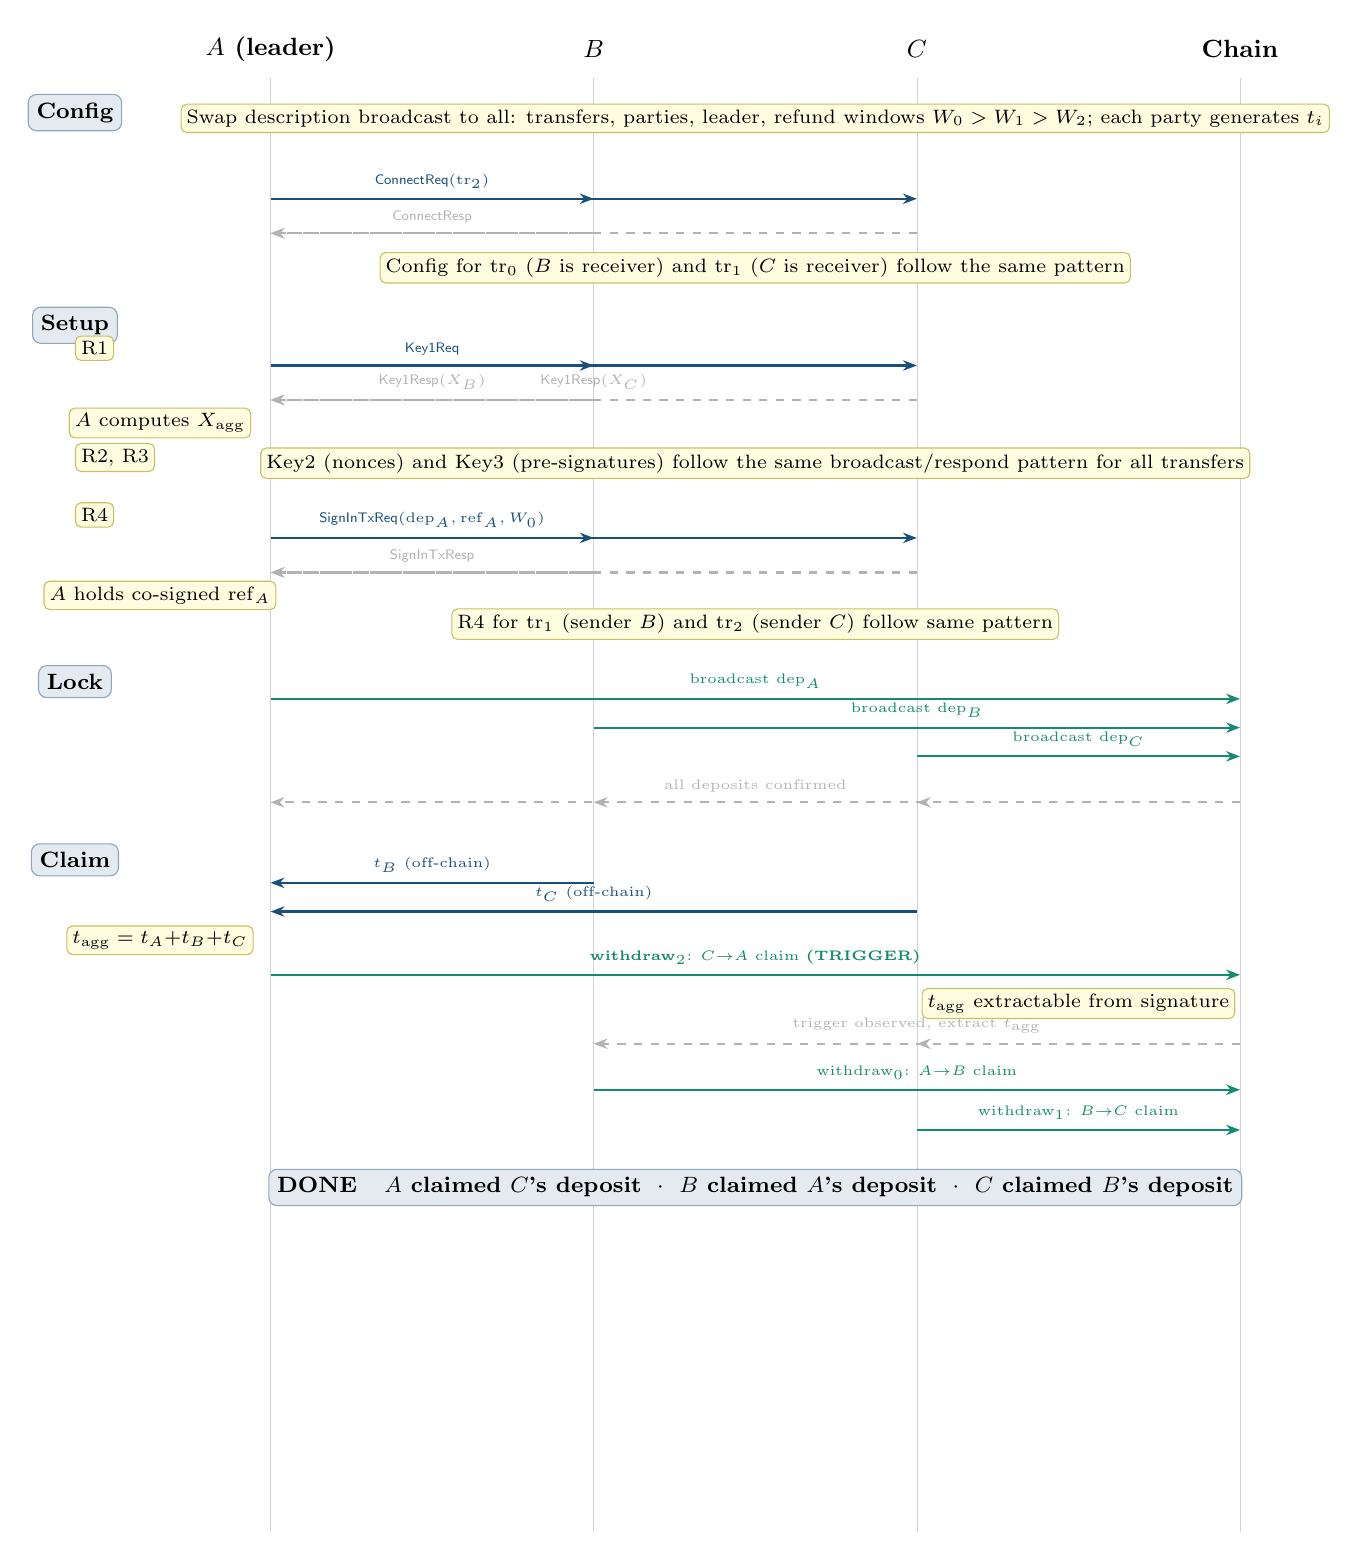
\begin{tikzpicture}[
  xscale=1.08, yscale=0.73,
  life/.style={very thin, gray!35},
  fwd/.style={-{Stealth[length=5pt]}, thick, protoblue},
  teal/.style={-{Stealth[length=5pt]}, thick, tealclaim},
  bwd/.style={-{Stealth[length=5pt]}, thick, dashed, gray!60},
  phase/.style={
    font=\footnotesize\bfseries, fill=protoblue!12,
    draw=protoblue!50, rounded corners=3pt, inner sep=3pt},
  note/.style={
    font=\scriptsize, fill=yellow!12,
    draw=yellow!50!gray, rounded corners=2pt, inner sep=2pt},
  hdr/.style={font=\small\bfseries},
]
  %% Lifelines
  \foreach \x/\n in {0/$A$~(leader), 3.8/$B$, 7.6/$C$, 11.4/Chain} {
    \node[hdr] at (\x, 0.3) {\n};
    \draw[life] (\x,-0.2) -- (\x,-25.5);
  }

  %% ─── CONFIG ─────────────────────────────────────────────────────────
  \node[phase] at (-2.3,-0.8) {Config};
  \node[note] at (5.7,-0.9)
    {Swap description broadcast to all: transfers, parties, leader, refund windows $W_0>W_1>W_2$; each party generates $t_i$};

  % tr2: A is receiver → sends ConnectReq
  \draw[fwd] (0,-2.3) -- node[above,font=\tiny] {\msg{ConnectReq}($\mathrm{tr}_2$)} (3.8,-2.3);
  \draw[fwd] (0,-2.3) -- (7.6,-2.3);
  \draw[bwd] (3.8,-2.9) -- node[above,font=\tiny] {\msg{ConnectResp}} (0,-2.9);
  \draw[bwd] (7.6,-2.9) -- (0,-2.9);

  % tr0, tr1 abbreviated
  \node[note] at (5.7,-3.5)
    {Config for $\mathrm{tr}_0$ ($B$ is receiver) and $\mathrm{tr}_1$ ($C$ is receiver) follow the same pattern};

  %% ─── SETUP: Round 1 ──────────────────────────────────────────────────
  \node[phase] at (-2.3,-4.5) {Setup};
  \node[note, anchor=west] at (-2.3,-4.9) {R1};

  % tr2, receiver = A
  \draw[fwd] (0,-5.2)  -- node[above,font=\tiny] {\msg{Key1Req}} (3.8,-5.2);
  \draw[fwd] (0,-5.2)  -- (7.6,-5.2);
  \draw[bwd] (3.8,-5.8) -- node[above,font=\tiny] {\msg{Key1Resp}$(X_B)$} (0,-5.8);
  \draw[bwd] (7.6,-5.8) -- node[above,font=\tiny] {\msg{Key1Resp}$(X_C)$} (0,-5.8);
  \node[note] at (-1.3,-6.2) {\scriptsize $A$ computes $\Xagg$};

  % R2/R3 abbreviated
  \node[note, anchor=west] at (-2.3,-6.8) {R2, R3};
  \node[note] at (5.7,-6.9)
    {Key2 (nonces) and Key3 (pre-signatures) follow the same broadcast/respond pattern for all transfers};

  %% ─── SETUP: Round 4 ──────────────────────────────────────────────────
  \node[note, anchor=west] at (-2.3,-7.8) {R4};

  % tr0: sender = A
  \draw[fwd] (0,-8.2)  -- node[above,font=\tiny] {\msg{SignInTxReq}$(\mathrm{dep}_A, \mathrm{ref}_A, W_0)$} (3.8,-8.2);
  \draw[fwd] (0,-8.2)  -- (7.6,-8.2);
  \draw[bwd] (3.8,-8.8) -- node[above,font=\tiny] {\msg{SignInTxResp}} (0,-8.8);
  \draw[bwd] (7.6,-8.8) -- (0,-8.8);
  \node[note] at (-1.3,-9.2) {\scriptsize $A$ holds co-signed $\mathrm{ref}_A$};

  % tr1 (sender B) and tr2 (sender C) abbreviated
  \node[note] at (5.7,-9.7)
    {R4 for $\mathrm{tr}_1$ (sender $B$) and $\mathrm{tr}_2$ (sender $C$) follow same pattern};

  %% ─── LOCK ────────────────────────────────────────────────────────────
  \node[phase] at (-2.3,-10.7) {Lock};

  \draw[teal] (0,-11.0)  -- node[above,font=\tiny] {broadcast $\mathrm{dep}_A$} (11.4,-11.0);
  \draw[teal] (3.8,-11.5) -- node[above,font=\tiny] {broadcast $\mathrm{dep}_B$} (11.4,-11.5);
  \draw[teal] (7.6,-12.0) -- node[above,font=\tiny] {broadcast $\mathrm{dep}_C$} (11.4,-12.0);

  \draw[bwd] (11.4,-12.8) -- node[above,font=\tiny] {all deposits confirmed} (0,-12.8);
  \draw[bwd] (11.4,-12.8) -- (3.8,-12.8);
  \draw[bwd] (11.4,-12.8) -- (7.6,-12.8);

  %% ─── CLAIM ───────────────────────────────────────────────────────────
  \node[phase] at (-2.3,-13.8) {Claim};

  % Non-leaders send secrets to A (off-chain)
  \draw[fwd] (3.8,-14.2) -- node[above,font=\tiny] {$t_B$ (off-chain)} (0,-14.2);
  \draw[fwd] (7.6,-14.7) -- node[above,font=\tiny] {$t_C$ (off-chain)} (0,-14.7);
  \node[note] at (-1.3,-15.2)
    {\scriptsize $\tagg = t_A{+}t_B{+}t_C$};

  % Leader broadcasts trigger
  \draw[teal] (0,-15.8) -- node[above,font=\tiny]
    {\textbf{withdraw}$_2$: $C{\to}A$ claim \textbf{(TRIGGER)}} (11.4,-15.8);
  \node[note] at (9.5,-16.3) {\scriptsize $\tagg$ extractable from signature};

  % Others observe trigger
  \draw[bwd] (11.4,-17.0) -- node[above,font=\tiny] {trigger observed, extract $\tagg$} (3.8,-17.0);
  \draw[bwd] (11.4,-17.0) -- (7.6,-17.0);

  % B and C broadcast their withdraws
  \draw[teal] (3.8,-17.8) -- node[above,font=\tiny]
    {withdraw$_0$: $A{\to}B$ claim} (11.4,-17.8);
  \draw[teal] (7.6,-18.5) -- node[above,font=\tiny]
    {withdraw$_1$: $B{\to}C$ claim} (11.4,-18.5);

  %% ─── DONE ────────────────────────────────────────────────────────────
  \node[phase] at (5.7,-19.5) {%
    DONE\quad $A$ claimed $C$'s deposit
    $\;\cdot\;$ $B$ claimed $A$'s deposit
    $\;\cdot\;$ $C$ claimed $B$'s deposit};
\end{tikzpicture}
\caption{Full happy-path trace for $N=3$, leader $= A$.
  Blue arrows: protocol (off-chain) messages.
  Teal arrows: on-chain transactions and chain-to-party notifications.
  Dashed arrows: responses.
  Config and Setup R1 for $\mathrm{tr}_0$ and $\mathrm{tr}_1$ follow the same
  pattern as shown for $\mathrm{tr}_2$.
  Setup R4 for $\mathrm{tr}_1$ and $\mathrm{tr}_2$ follows the same pattern
  as shown for $\mathrm{tr}_0$.
  Rounds R2 and R3 follow the broadcast/respond pattern noted inline.}
\label{fig:trace}
\end{figure}

% ─────────────────────────────────────────────────────────────────────────────
\section{Example Trace: $N = 3$, Refund Path}

\noindent
\textbf{Parties:} $A = P_0$ (leader), $B = P_1$, $C = P_2$.\\
\textbf{Cycle:} $A \to B \to C \to A$.\\
\textbf{Scenario:} $B$ withholds $t_B$ during Claim.
$A$ cannot assemble $\tagg$ and does not broadcast the trigger.
All parties wait out their respective refund windows and reclaim their
deposits.

The full sequence diagram is shown in Figure~\ref{fig:trace-refund}.

\begin{figure}[p]
\centering
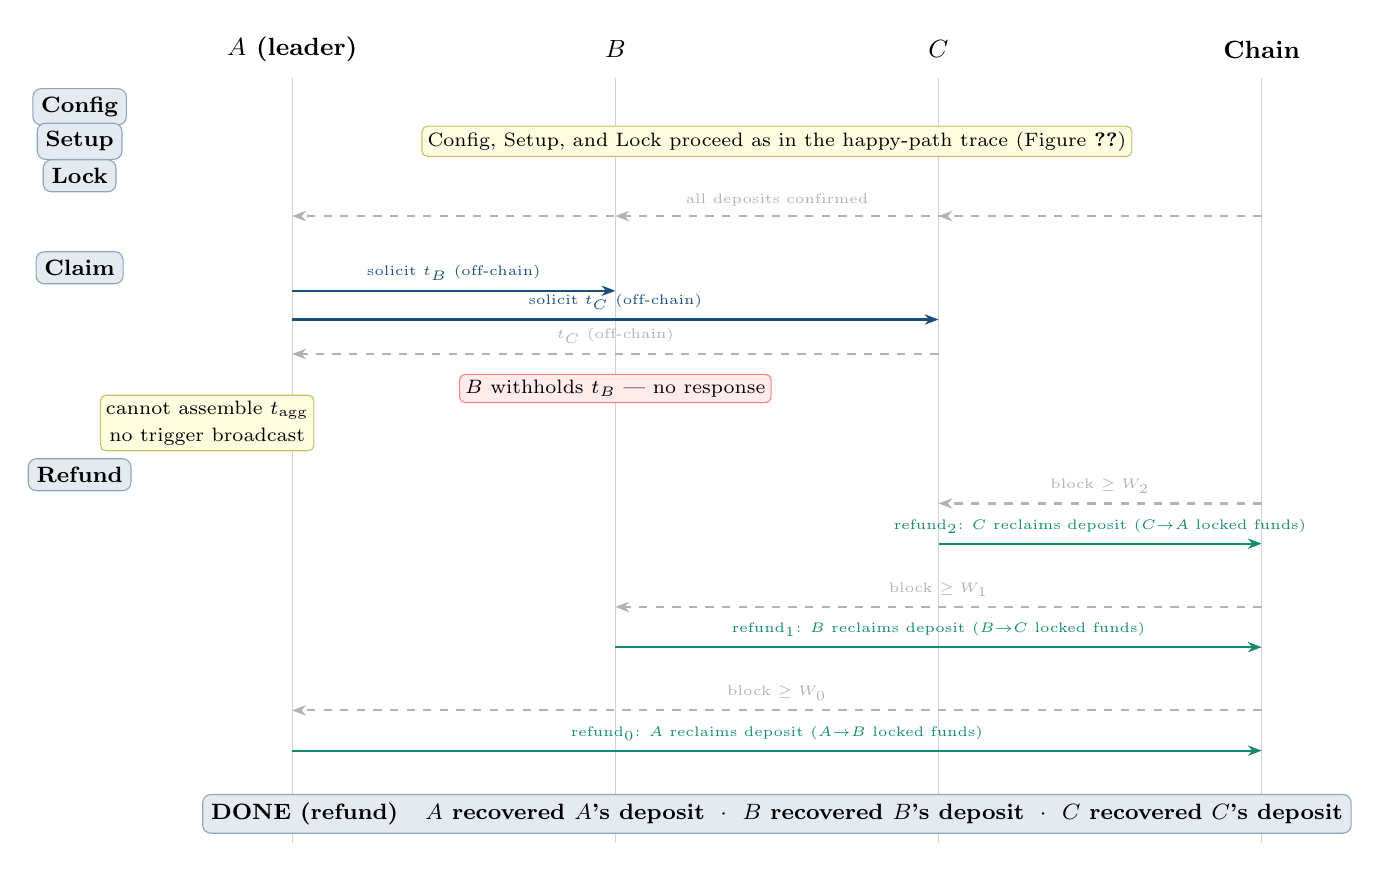
\begin{tikzpicture}[
  xscale=1.08, yscale=0.73,
  life/.style={very thin, gray!35},
  fwd/.style={-{Stealth[length=5pt]}, thick, protoblue},
  teal/.style={-{Stealth[length=5pt]}, thick, tealclaim},
  bwd/.style={-{Stealth[length=5pt]}, thick, dashed, gray!60},
  phase/.style={
    font=\footnotesize\bfseries, fill=protoblue!12,
    draw=protoblue!50, rounded corners=3pt, inner sep=3pt},
  note/.style={
    font=\scriptsize, fill=yellow!12,
    draw=yellow!50!gray, rounded corners=2pt, inner sep=2pt},
  bad/.style={
    font=\scriptsize, fill=red!8,
    draw=red!50, rounded corners=2pt, inner sep=2pt},
  hdr/.style={font=\small\bfseries},
]
  %% Lifelines
  \foreach \x/\n in {0/$A$~(leader), 3.8/$B$, 7.6/$C$, 11.4/Chain} {
    \node[hdr] at (\x, 0.3) {\n};
    \draw[life] (\x,-0.2) -- (\x,-13.5);
  }

  %% ─── CONFIG / SETUP / LOCK (abbreviated) ────────────────────────────
  \node[phase] at (-2.5,-0.7) {Config};
  \node[phase] at (-2.5,-1.3) {Setup};
  \node[phase] at (-2.5,-1.9) {Lock};
  \node[note] at (5.7,-1.3)
    {Config, Setup, and Lock proceed as in the happy-path trace
     (Figure~\ref{fig:trace})};

  \draw[bwd] (11.4,-2.6) -- node[above,font=\tiny] {all deposits confirmed}
    (0,-2.6);
  \draw[bwd] (11.4,-2.6) -- (3.8,-2.6);
  \draw[bwd] (11.4,-2.6) -- (7.6,-2.6);

  %% ─── CLAIM: B withholds ──────────────────────────────────────────────
  \node[phase] at (-2.5,-3.5) {Claim};

  \draw[fwd] (0,-3.9) -- node[above,font=\tiny] {solicit $t_B$ (off-chain)}
    (3.8,-3.9);
  \draw[fwd] (0,-4.4) -- node[above,font=\tiny] {solicit $t_C$ (off-chain)}
    (7.6,-4.4);

  \draw[bwd] (7.6,-5.0) -- node[above,font=\tiny] {$t_C$ (off-chain)}
    (0,-5.0);

  \node[bad] at (3.8,-5.6) {$B$ withholds $t_B$ --- no response};

  \node[note] at (-1.0,-6.2)
    {\shortstack{\scriptsize cannot assemble $\tagg$\\\scriptsize no trigger broadcast}};

  %% ─── REFUND ──────────────────────────────────────────────────────────
  \node[phase] at (-2.5,-7.1) {Refund};

  % W_2: C's window opens first
  \draw[bwd] (11.4,-7.6) -- node[above,font=\tiny] {block $\geq W_2$}
    (7.6,-7.6);
  \draw[teal] (7.6,-8.3) -- node[above,font=\tiny]
    {refund$_2$: $C$ reclaims deposit ($C{\to}A$ locked funds)} (11.4,-8.3);

  % W_1: B's window
  \draw[bwd] (11.4,-9.4) -- node[above,font=\tiny] {block $\geq W_1$}
    (3.8,-9.4);
  \draw[teal] (3.8,-10.1) -- node[above,font=\tiny]
    {refund$_1$: $B$ reclaims deposit ($B{\to}C$ locked funds)} (11.4,-10.1);

  % W_0: A's window opens last
  \draw[bwd] (11.4,-11.2) -- node[above,font=\tiny] {block $\geq W_0$}
    (0,-11.2);
  \draw[teal] (0,-11.9) -- node[above,font=\tiny]
    {refund$_0$: $A$ reclaims deposit ($A{\to}B$ locked funds)} (11.4,-11.9);

  %% ─── DONE ────────────────────────────────────────────────────────────
  \node[phase] at (5.7,-13.0) {%
    DONE (refund)\quad $A$ recovered $A$'s deposit
    $\;\cdot\;$ $B$ recovered $B$'s deposit
    $\;\cdot\;$ $C$ recovered $C$'s deposit};
\end{tikzpicture}
\caption{Refund-path trace for $N=3$, leader $= A$.
  $B$ withholds $t_B$; $A$ cannot assemble $\tagg$ and no trigger is
  broadcast.
  $C$'s refund window $W_2$ opens first; $B$'s $W_1$ next; $A$'s $W_0$
  last.
  Each party independently monitors the chain and broadcasts their refund tx
  as soon as their window opens.
  No principal is lost.
  Style conventions as in Figure~\ref{fig:trace}.}
\label{fig:trace-refund}
\end{figure}

% ─────────────────────────────────────────────────────────────────────────────
\section{Scope and Open Issues}

\begin{itemize}
  \item \textbf{Non-cyclic swaps} (separate input and output parties):
    the staggered window invariant does not straightforwardly generalise and
    remains an open design problem.
    Out of scope for this specification.
  \item \textbf{Leader election:}
    the leader is assumed pre-determined.
    A commit-reveal randomness scheme (hash all nonces, take index
    $H(\ldots)\bmod N$) can be used but is not part of the core protocol.
  \item \textbf{Cross-chain finality:}
    the definition of ``confirmed'' for each blockchain is chain-specific
    and is treated as an oracle input to this protocol.
  \item \textbf{Cryptographic soundness:}
    the adaptor signature scheme, the MuSig2 multi-signature scheme, and their
    combination are assumed correct and secure.
\end{itemize}

\bibliographystyle{plain}
\bibliography{references}

\end{document}
